\chapter{Continual Learning}

\section{Introduction}

\subsection{Humans and Memory}
Human intelligence is characterized by its remarkable ability to learn from sequences of events and tasks without erasing prior compe-
tencies. A person may first learn to distinguish cats from dogs, and later learn to distinguish cars from boats, while still retaining the
ability to correctly identify a dog. \textbf{This sequence learning capability} is central to human cognition: new knowledge is integrated without
completely overwriting what came before

\begin{figure}[H]
    \centering
    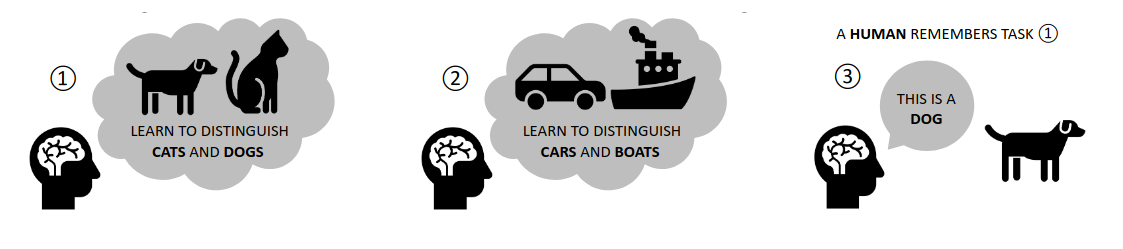
\includegraphics[width=0.75
    \textwidth]{images/CL1.png}
    \label{fig:MHA2}
\end{figure}

\subsection{Neural Networks and Catastrophic Forgetting}
Artificial Neural Networks behave differently. When trained on tasks sequentially, they tend to forget earlier ones: a phenomenon
known as \textbf{catastrophic forgetting}. After learning Task 1 (cats vs. dogs) and then Task 2 (cars vs. boats), a neural network may incorrectly
classify a dog as a car. Performance on the most recent task is preserved, while accuracy on previous tasks sharply deteriorates. This
happens because networks show an \textbf{intrinsic bias toward recently learned tasks}, making them less versatile in long-term, incremental
learning scenarios.

This issue is closely connected to our earlier discussions about \textbf{PEFT (Parameter-Efficient Fine-Tuning)}. When performing \textbf{full fine-tuning
(FFT)}, we adjust all model parameters, which can drastically alter the internal representations. Such drastic parameter changes can
cause the model to forget crucial features learned earlier, resulting in a loss of generalization (another form of catastrophic forgetting).
PEFT techniques, by contrast, aim to limit parameter updates to avoid this destructive overwrite.

\begin{figure}[H]
    \centering
    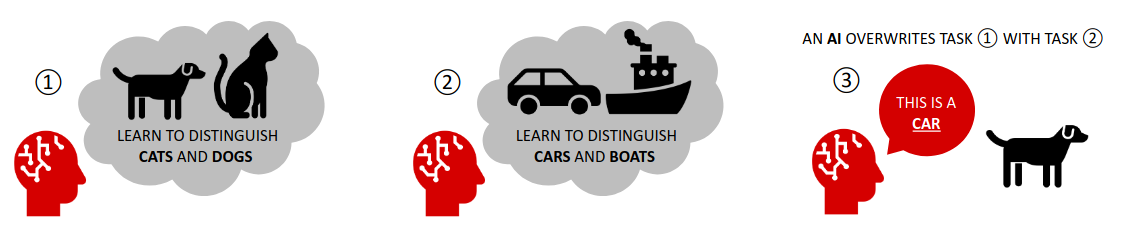
\includegraphics[width=0.75
    \textwidth]{images/CL2.png}
    \label{fig:MHA2}
\end{figure}

\subsection{Humans VS Neural Network}
\begin{wrapfigure}{r}{0.4\textwidth}
    \centering
    \vspace{-10pt}
    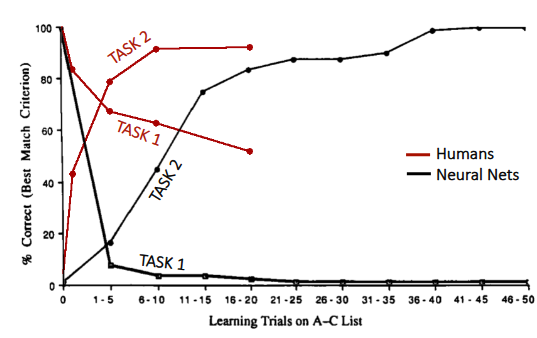
\includegraphics[width=\linewidth]{images/CL3.png}
    \label{fig:Scaled Dot Product Attention}
    \vspace{-10pt}
\end{wrapfigure}
The distinction between human forgetting and neural-network forgetting was highlighted
early in psychology. In 1959, \textbf{Barnes and Underwood} examined how humans learn two
sequential tasks. Participants learned word pairs such as home-star and field-sky (Task 1),
then learned modified pairs like home-field and field-car (Task 2). Results showed that hu-
mans do forget some of the initial associations: performance declines on Task 1 while im-
proving on Task 2. However, this degradation is \textbf{gradual}, not destructive.

In 1989, \textbf{McCloskey and Cohen} repeated the same two-task experiment using artificial
neural networks. Their findings were striking: networks did not simply become slightly worse on Task 1, they lost the ability to perform
it almost entirely after just a few learning steps on Task 2. The drop in performance was rapid, severe, and complete. This is why re-
searchers call it \textbf{catastrophic} forgetting: the forgetting is not merely present but overwhelmingly destructive, reducing earlier learning
to effectively zero.

\subsection{Why Do Neural Networks Forget?}
Catastrophic forgetting arises primarily from optimization using \textbf{gradient descent}. A neural
network is defined by its parameters $W$. Training on Task~A moves the parameters from a
random initialization $W_0$ to a solution $W_A$ that yields low error for that task. When the
network is later trained on Task~B, gradient descent modifies these same parameters, pushing
them toward another optimum $W_B$, often far from the region where Task~A performed well.
Task~A’s performance therefore collapses.  

Although neural networks are often \textbf{over-parameterized}, meaning that joint solutions $W_{A+B}$
capable of solving both tasks likely exist, standard optimization has no built-in mechanism to
preserve old knowledge. SGD simply follows the gradient of the new task, even when this drives
the model away from earlier solutions.

\begin{figure}[H]
    \centering
    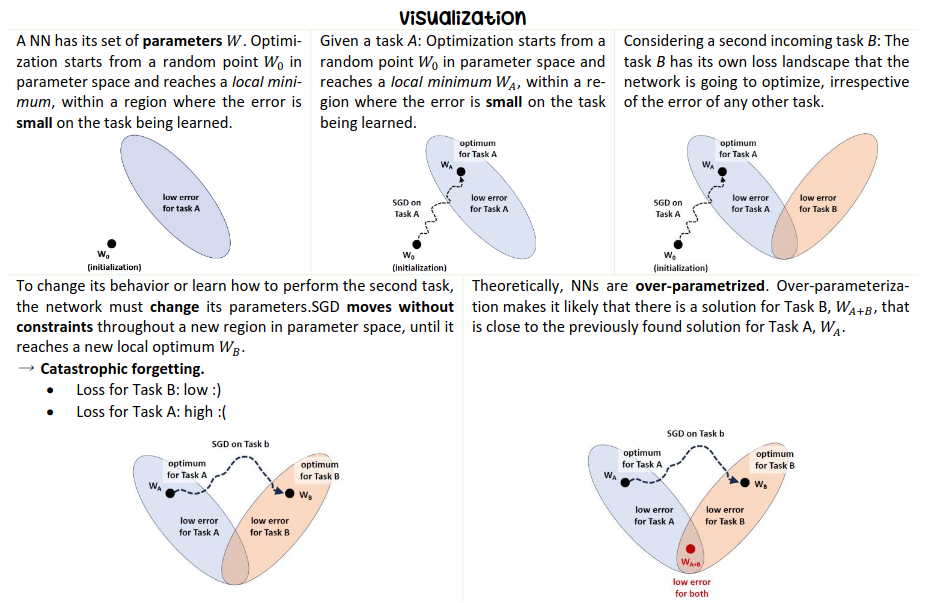
\includegraphics[width=1
    \textwidth]{images/CL4.png}
    \label{fig:MHA2}
\end{figure}

\textbf{Continual Learning (CL)} aims to overcome catastrophic forgetting by training models on streams of evolving data while preserving prior
knowledge. The goal is to constrain learning so that updates for Task B do not destroy the low-error region for Task A, even though the
model no longer has access to Task-A training examples. Achieving this without retraining from scratch is one of the central challenges
in continual learning.

CL has become a rapidly growing research area, with interest from both academia and indus-
try. Startups and large companies are exploring CL to build AI systems that adapt over time,
remain versatile, and avoid the catastrophic knowledge loss observed in standard neural net-
works. Trends in publications and search interest demonstrate increasing attention to this
field.

\subsection{A Common Continual Learning Scenario}
In a typical continual learning (CL) setting, a classification problem is divided into
$T$ sequential tasks. During each task $t \in \{1, \dots, T\}$, the model receives input
samples $x$ and labels $y$ drawn i.i.d.\ from a distribution $D_t$. A classic example is the
Split MNIST protocol, where the MNIST dataset is partitioned into 5 tasks, each containing two
digits (e.g., Task~1: 0/1, Task~2: 2/3, \dots, Task~5: 8/9). The model learns each task in
sequence, and past data are assumed to become unavailable as soon as training proceeds to the
next task.

\begin{figure}[H]
    \centering
    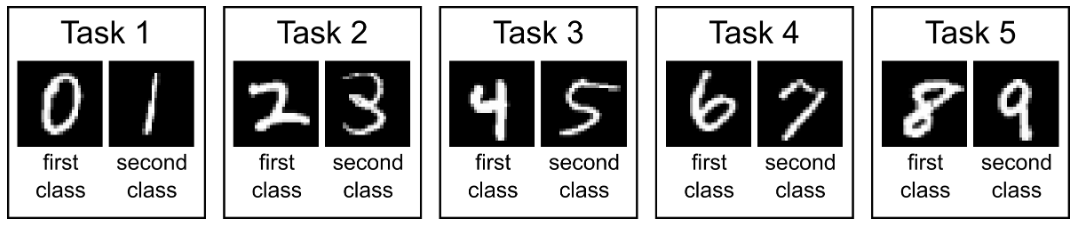
\includegraphics[width=0.8
    \textwidth]{images/CL5.png}
    \label{fig:MHA2}
\end{figure}
In scenarios such as \textbf{Task-IL} (Task-Incremental Learning), at the model is told which task an input
belongs to, for example, whether the image contains the first or the second class of the
current pair. A single function $f_\theta$ must be optimized sequentially, task after task,
over time.

This setting is important both in research and in industry. Real-world systems often face
streams of continuously arriving data, and retraining from scratch (joint training on all
past and present data) is extremely expensive or outright infeasible. Continual learning
methods aim to avoid this inefficiency.

\subsection{The Common Objective in CL}
The goal of continual learning is clear: at any point in training, the model should correctly
classify inputs from all tasks observed so far. Formally, at time $t_c$, we aim to minimize
the cumulative loss:
\[
\arg \min_{\theta} \sum_{t=1}^{t_c} \mathcal{L}_t
\quad \text{where} \quad
\mathcal{L}_t \equiv \mathbb{E}_{(x,y)\sim D_t}\bigl[\ell\bigl(y, f_\theta(x)\bigr)\bigr].
\]

The key challenge is that the data from previous tasks $D_1, \dots, D_{t_c-1}$ are assumed to
be \textbf{unavailable}. The model must find the best parameters for all tasks using only the current
dataset $D_{t_c}$. This makes the problem extremely challenging: we want the model to behave
well on tasks A and B while only seeing data from B.

Gradient descent makes this even more difficult because it is a \textbf{greedy} optimizer. At each
step, it changes parameters to reduce the loss on the current data subset. There is no
guarantee that these updates remain compatible with earlier tasks. In fact, as seen earlier,
vanilla fine-tuning almost always overwrites previously acquired knowledge.

\subsection{A NAÏVE Baseline: Joint Training}
One obvious solution would be to avoid forgetting entirely: simply retrain the model jointly on all available data from Tasks A and B.
This guarantees the best performance but is extremely inefficient and unrealistic, especially when data continue to arrive over time.
Continual learning explicitly avoids this “retrain-everything” approach by assuming that past data cannot be stored indefinitely.

\subsection{Elastic Weight Consolidation (EWC)}
One of the first influential methods developed to mitigate catastrophic forgetting is
\textbf{Elastic Weight Consolidation (EWC)}, introduced by Kirkpatrick et al.\ in 2017. EWC is
inspired by biological mechanisms, specifically the concept of \textbf{synaptic consolidation}
in the brain.

Humans do experience forgetting when learning tasks sequentially, but this forgetting is mild
and gradual, not destructive. This difference is partly due to biological mechanisms such as
\textbf{synaptic consolidation}: when humans learn something important, the corresponding neural
connections become more stable and resistant to change. As a result, when a new task is
learned, the brain does not overwrite earlier knowledge but adjusts only the connections that
are still flexible. In other words, humans have a natural form of \textbf{selective plasticity} that
preserves crucial information while continuing to learn.

Neural networks lack this mechanism by default. During gradient descent, all parameters remain
highly plastic and can be modified drastically. So when the model learns the second task, it
unintentionally overwrites parameter configurations that were essential for the first one.
This is why forgetting in humans is limited, while in machines it becomes catastrophic: in
just a few learning steps, the model can lose almost all ability to perform the earlier task.

So, in the brain:
\begin{compactitemize}
    \item biological \textbf{plasticity} allows the nervous system to adapt while preserving important
    synaptic strengths;
    \item \textbf{synapses} crucial to previously learned tasks become less plastic, protecting old
    memories from being overwritten.
\end{compactitemize}

EWC transfers this intuition to neural networks: parameters that were important for past tasks
should not change too much when learning a new one. It does so by adding a \textbf{quadratic penalty}
to the loss function that acts like an elastic "spring", pulling parameters back toward
their old values.

So, it can be imagined as a spring \textbf{anchoring} the parameters to the previous solution, hence
the name \textbf{elastic}. Importantly, the stiffness of this spring should not be the same for
all parameters; rather, \textbf{it should be greater} for those parameters that \textbf{matter most} to the
performance during Task~A.

\subsection{The EWC Loss Function}
When learning Task~B, the total loss optimized by EWC is:
\[
\mathcal{L}(\theta)
=
\mathcal{L}_B(\theta)
+
\sum_i \frac{\lambda}{2}
F_i \bigl(\theta_i - \theta^{*}_{A,i}\bigr)^2.
\]
\newpage
\begin{wrapfigure}{r}{0.4\textwidth}
    \centering
    \vspace{-10pt}
    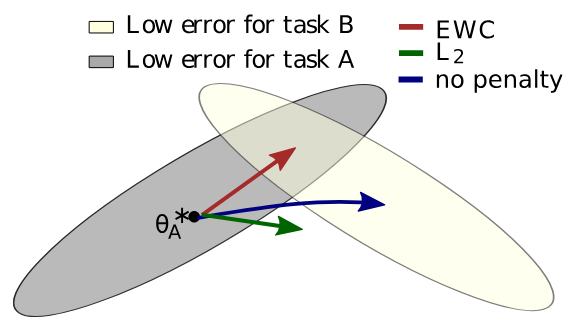
\includegraphics[width=\linewidth]{images/CL6.png}
    \label{fig:Scaled Dot Product Attention}
    \vspace{-10pt}
\end{wrapfigure}
Here:
\begin{compactitemize}
    \item $\mathcal{L}_B(\theta)$ is the standard loss for Task~B (typically cross-entropy, for
    classification);
    \item $\theta^{*}_A$ are the optimal parameters for Task~A;
    \item $F_i$ is the estimated importance of parameter $i$ for Task~A;
    \item $\lambda$ is a scaling hyperparameter balancing plasticity vs.\ stability.
\end{compactitemize}

Intuitively, this loss enforces two objectives:
\begin{enumerate}
    \item \textbf{learn Task~B well} by minimizing $\mathcal{L}_B$;
    \item \textbf{stay close to the Task~A solution} by minimizing the weighted squared distance between
    $\theta$ and $\theta^{*}_A$.
\end{enumerate}

If we momentarily ignore the importance weights and the scaling factors, the second term
essentially becomes $\bigl(\theta_i - \theta^{*}_{A,i}\bigr)^2$, which is simply the \text{squared
Euclidean distance} from the old optimum. In practice, this term encourages the updated
parameters to stay close to the values that previously worked well for Task~A, keeping the
new solution within its neighborhood.

\subsection{The Role of $F_i$}
The parameter-specific factor $F_i$:
\begin{compactitemize}
    \item is \textbf{not learnable};
    \item depends on the importance of each parameter for Task~A;
    \item controls how strongly that parameter should resist change.
\end{compactitemize}

If $F_i \approx 0$, the parameter is free to adapt to Task~B. If $F_i$ is large, the ``spring''
becomes stiff, preventing the parameter from moving far from its Task~A optimum.

\subsection{The Role of $\lambda$}
$\lambda$ adjusts the overall weight of the penalty. It controls the global trade-off between
retaining old knowledge (Task~A) and acquiring new knowledge (Task~B).

\subsection{Estimating Parameter Importance: The Fisher Information Matrix}
To compute the importance weights $F_i$, EWC uses the \textbf{diagonal of the empirical Fisher
Information Matrix (FIM)} computed at the Task~A optimal parameters:
\[
\mathcal{I}_{\theta_A^*}
=
\frac{1}{N}
\sum_{i=1}^{N}
\bigl[
\nabla_\theta \log p(x_A^{(i)} \mid \theta_A^*)
\bigr]
\bigl[
\nabla_\theta \log p(x_A^{(i)} \mid \theta_A^*)
\bigr]^{\top}.
\]

Because EWC uses only the diagonal, $F_i$ becomes:
\[
F_i
=
\frac{1}{N}
\sum_{k=1}^{N}
\left(
\frac{\partial \mathcal{L}(x_k)}{\partial \theta_i}
\right)^2.
\]

This quantity can be computed from squared gradients: simple, cheap, and efficient.

\subsection{Why Does Make Sense?}
The gradient magnitude $\left|\frac{\partial \mathcal{L}(x_i)}{\partial \theta_i}\right|$ measures how
sensitive the loss is to changes in parameter $\theta_i$:
\begin{compactitemize}
    \item if the gradient is \textbf{small}, perturbing $\theta_i$ barely affects performance
    $\rightarrow$ the parameter is not crucial $\rightarrow$ small penalty;
    \item if the gradient is \textbf{large}, even small changes harm performance
    $\rightarrow$ the parameter is important $\rightarrow$ large penalty.
\end{compactitemize}

Since EWC squares the gradient:
\begin{enumerate}
    \item the sign does not matter (only magnitude);
    \item bigger sensitivities are penalized more strongly.
\end{enumerate}

\subsection{Second-Derivative Interpretation}
\begin{wrapfigure}{r}{0.3\textwidth}
    \centering
    \vspace{-10pt}
    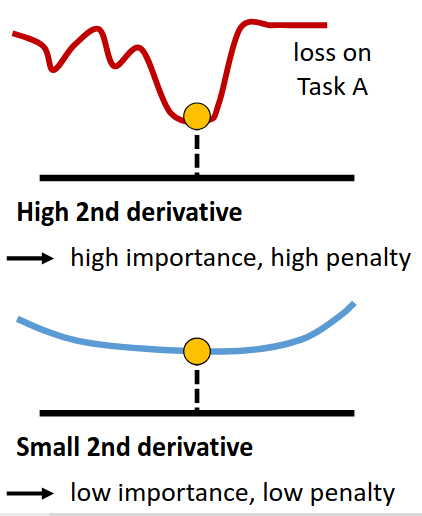
\includegraphics[width=\linewidth]{images/CL7.png}
    \label{fig:Scaled Dot Product Attention}
    \vspace{-10pt}
\end{wrapfigure}
There is also a geometric interpretation. Near a minimum, the second derivative of the loss
describes the curvature of the local region:
\begin{compactitemize}
    \item \textbf{high curvature} (sharp minimum) $\rightarrow$ loss increases rapidly
    $\rightarrow$ the corresponding weight must not move
    $\rightarrow$ high Fisher information $\rightarrow$ strong penalty.
    Few degrees of freedom;
    \item \textbf{low curvature} (flat minimum) $\rightarrow$ weight can change with little harm
    $\rightarrow$ low Fisher information $\rightarrow$ weak penalty.
    Many degrees of freedom.
\end{compactitemize}

Thus, the FIM acts as a proxy for the local geometry of the loss landscape around
$\theta_A^{*}$. This captures how many "degrees of freedom" the model has when adapting
to Task~B without corrupting Task~A.

\section{Continual Learning}

\subsection{Continual Learning Benchmarks}
Continual Learning (CL) methods are traditionally evaluated on simplified and highly controlled
image-classification benchmarks. These settings are designed to isolate specific challenges of
learning over time while avoiding confounding factors such as dataset noise or large-scale
training costs.

\begin{compactitemize}
    \item A common family of benchmarks is based on sequential tasks. For example, in \textbf{Sequential
    MNIST}, the classification problem is split into multiple subtasks: Task~1 consists of
    distinguishing digits 0 vs.\ 1, Task~2 focuses on digits 2 vs.\ 3, and so on. Similarly,
    \textbf{Sequential CIFAR} defines a sequence of binary classification problems, such as
    airplane vs.\ car in Task~1 and bird vs.\ cat in Task~2.
    
    \item Other benchmarks introduce structured changes to the input distribution. In \textbf{Rotated
    MNIST}, each task presents digit images rotated by a different angle, requiring the model
    to cope with domain shifts.
    
    \item In \textbf{Permuted MNIST}, every task applies a different fixed pixel permutation, generating
    distinct yet related classification problems.
\end{compactitemize}

Although more realistic benchmarks involving long and complex sequences of tasks exist, they
are often \textbf{computationally demanding}. For this reason, the community still relies heavily on
these abstract yet manageable setups.

\subsection{Evaluation Protocol}
Evaluation in Continual Learning typically relies on predefined train/test splits for each
task.

\begin{compactitemize}
    \item During \textbf{training}, tasks are presented sequentially: the model learns one task at a time,
    without revisiting data from previous tasks. Multiple training epochs per task are usually
    allowed to ensure that the model can fit each new task adequately.

    \item In the \textbf{testing} phase, the model is evaluated jointly on all test sets from every task
    encountered so far, regardless of order. This provides a measure of how well the model retains
    past knowledge while learning new information. Multiple epochs are usually allowed on each
    task, so that the model can fit the current task well.

\end{compactitemize}

A significant limitation of current CL research is the lack of unified hyperparameter tuning
protocols. Cross-validation and hyperparameter search strategies vary widely across studies,
making reproducibility and fair comparison challenging. Unfortunately, no established and
common practices already exist.

\subsection{Metrics}
The most commonly used metric in Continual Learning is \textbf{Average Accuracy (ACC)}. Let
$R_{i,j}$ denote the accuracy on task $t_j$ after the model has finished learning task $t_i$.
Once all $T$ tasks have been learned, ACC is defined as:
\[
\text{ACC}
=
\frac{1}{T}
\sum_{i=1}^{T}
R_{T,i}.
\]

This provides an overall assessment of the model’s performance on all tasks after the final
task has been trained. It can also be computed at intermediate points to track performance
progression.

Beyond ACC, other metrics are sometimes adopted, such as \textbf{Backward Transfer (BWT)},
which measures how much learning new tasks influences performance on old ones, and
\textbf{Forward Transfer (FWT)}, which measures whether learning earlier tasks helps
generalize to future ones. These were introduced by Lopez-Paz et al.\ in
\emph{Gradient Episodic Memory for Continual Learning}.

\subsection{Evaluation and Metrics}
\begin{figure}[H]
    \centering
    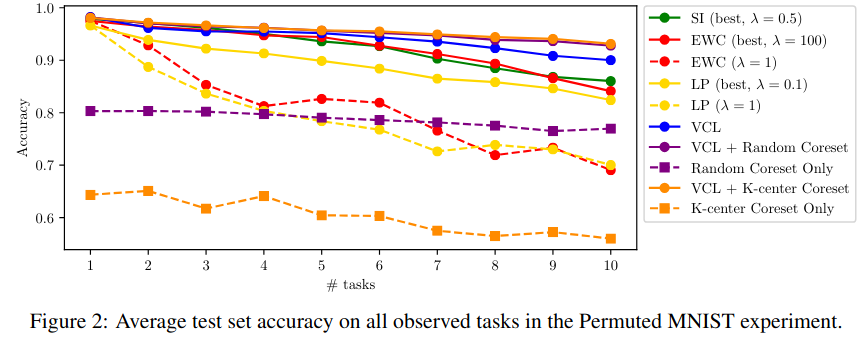
\includegraphics[width=0.9
    \textwidth]{images/CL8.png}
    \label{fig:MHA2}
\end{figure}

We can use plots like this to visualize the accuracy achieved on different tasks (shown on the x-axis) by various models. A common
pattern emerges: accuracy tends to decrease as the number of learned tasks grows. This is intuitive: each additional task increases the
range of concepts the model must recognize, and managing a larger set of tasks typically leads to progressively worse performance

\subsection{Evaluation Scenarios}
Continual Learning scenarios can differ significantly depending on what information is
available at test time and how tasks are defined. Three scenarios are most commonly
considered:

\begin{enumerate}
    \item \textbf{Task-Incremental Learning (Task-IL):}  
    In Task-IL, the model learns each task separately. During testing, the
    \textbf{identity of the task} associated with each input example \textbf{is provided}. This
    allows the system to select the appropriate output head or sub-module for that task.
    Task-IL is therefore the simplest scenario, as the model does not need to infer which
    task the test example belongs to.

    \begin{center}
        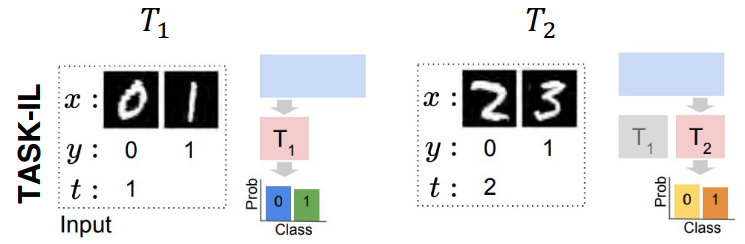
\includegraphics[width=0.6\textwidth]{images/CL9}
    \end{center}

    \item \textbf{Class-Incremental Learning (Class-IL):}  
    As in Task-IL, training occurs on one task at a time. However, at test time,
    \textbf{task identity is not given}. The model must predict the correct class among
    all classes observed so far. This setting is significantly more challenging, as it
    requires the model to integrate all knowledge accumulated across tasks into a unified
    classifier.

    \begin{center}
        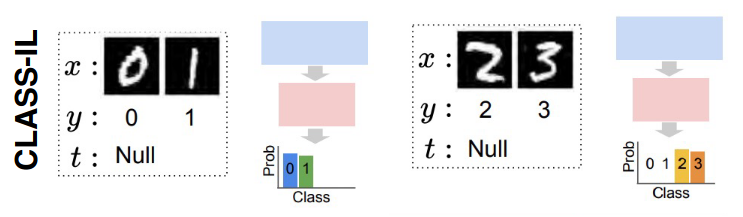
\includegraphics[width=0.6\textwidth]{images/CL10}
    \end{center}

    \item \textbf{Domain-Incremental Learning (Domain-IL):}  
    In Domain-IL, \textbf{the set of classes remains constant across tasks, but the input
    distribution changes}. Each task introduces a domain shift, such as image rotations or
    pixel permutations. The model must adapt to the new domain while preserving performance
    on the previous ones.

    \begin{center}
        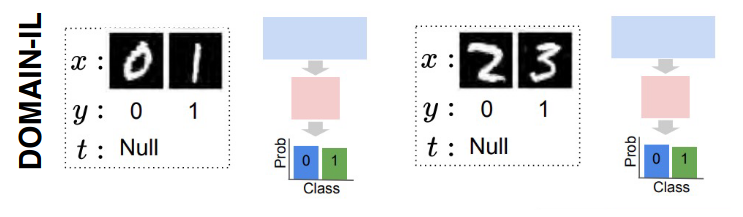
\includegraphics[width=0.6\textwidth]{images/CL11}
    \end{center}
\end{enumerate}

\subsection{Other Scenario in the Literature}

Additional scenarios broaden the conceptual space of Continual Learning.

$\rightarrow$ \textbf{General Continual Learning (GCL)} removes the notion of discrete tasks
entirely. Instead, the data distribution evolves smoothly over time, and the learner must
adapt continuously.
\begin{wrapfigure}{r}{0.3\textwidth}
    \centering
    \vspace{-10pt}
    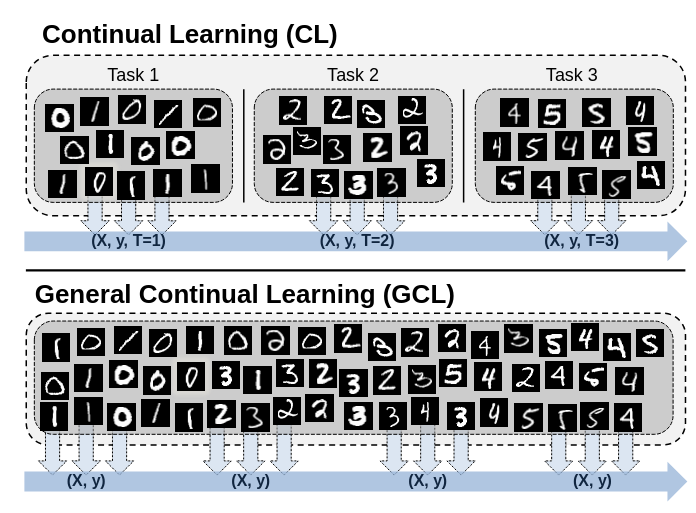
\includegraphics[width=\linewidth]{images/CL12.png}
    \label{fig:Scaled Dot Product Attention}
    \vspace{-10pt}
\end{wrapfigure}
$\rightarrow$ \textbf{Online Class-IL} and \textbf{Online Task-IL} impose stricter constraints
by allowing only a single pass (one epoch) over each task’s data, making the setting closer to
realistic streaming data scenarios.

$\rightarrow$ \textbf{Continual semi-supervised} or \textbf{self-supervised learning} extends
the problem to cases where labels are partially available or completely absent.

$\rightarrow$ \textbf{Data-Incremental Learning (Data-IL)} assumes that the set of classes is
fixed, and tasks correspond to different, possibly sequential partitions of the dataset.

In this course, the focus is on \textbf{Class-Incremental Learning}, as it is the most widely
studied and arguably the most difficult setting.

\subsection{A Taxonomy of Continual Learning Approaches}
\begin{wrapfigure}{r}{0.4\textwidth}
    \centering
    \vspace{-10pt}
    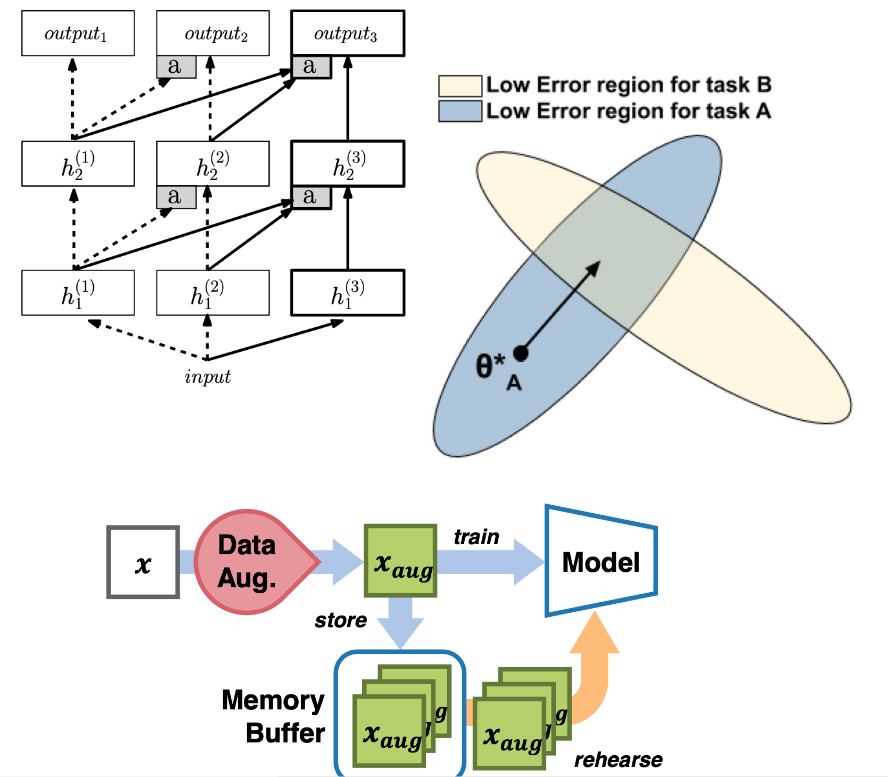
\includegraphics[width=\linewidth]{images/CL13.png}
    \label{fig:Scaled Dot Product Attention}
    \vspace{-10pt}
\end{wrapfigure}

CL methods are commonly grouped into three categories:

(A) \textbf{Architectural Methods}: These approaches allocate dedicated sub-networks or
components for different tasks. They often achieve excellent performance but typically
require increasing memory or model size as tasks accumulate.

(B) \textbf{Regularization Methods}: These introduce additional loss terms to prevent the
model from altering parameters critical for previously learned tasks. Examples include
weight-importance methods (e.g., Elastic Weight Consolidation) and knowledge
distillation--based approaches. They maintain bounded memory requirements and scale well
to long task sequences.

(C) \textbf{Replay Methods}: Replay approaches store selected examples from previous tasks in
a memory buffer. These samples are replayed during training on new tasks to prevent
forgetting. Replay is effective and conceptually straightforward, but performance generally
increases with the size of the memory buffer, making memory constraints a practical issue.

\section{(A) Architectural Methods}

\subsection{Weight Sharing}
A major source of \textbf{catastrophic forgetting} in neural networks is the \textbf{shared set of parameters} across multiple tasks. When a model learns
a new task, updates applied during training can overwrite the optimal parameter configuration that was previously learned for past
tasks. This \textbf{inter-task interference} arises because all incremental tasks are forced to share a single parameter space, making it difficult
to retain earlier knowledge.

The central question in Continual Learning is: how can we mitigate this interference and preserve past knowledge while still learning
new tasks effectively?

\subsection{Architectural Approaches}

One strategy to address inter-task interference is through \textbf{architectural methods}, which allocate distinct sub-models or task-specific
parameters for each task. The main idea is to \textbf{add new parameters for new tasks}, effectively isolating them from those used in previous
tasks. By doing so, the parameters for earlier tasks can be fixed, ensuring \textbf{maximal stability}.

\subsection{Progressive Neural Networks (PNN)}
\begin{wrapfigure}{r}{0.25\textwidth}
    \centering
    \vspace{-10pt}
    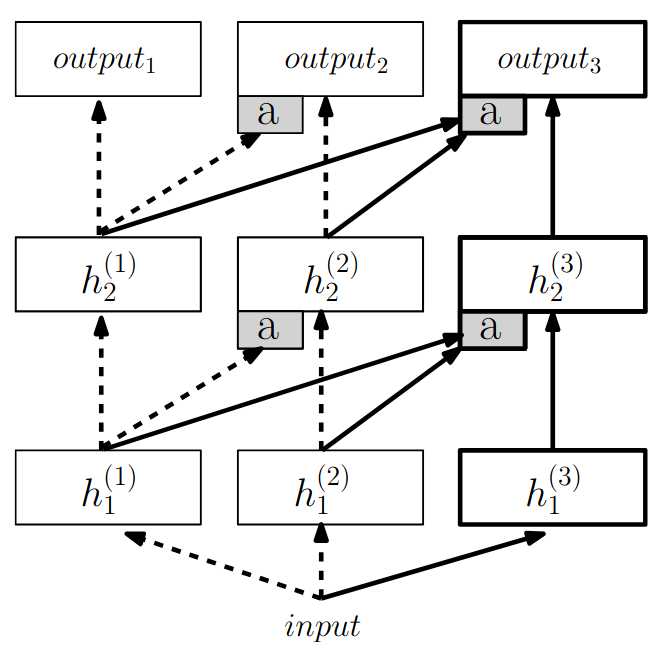
\includegraphics[width=\linewidth]{images/CL14.png}
    \label{fig:Scaled Dot Product Attention}
    \vspace{-10pt}
\end{wrapfigure}
An influential example of architectural approaches is \textbf{Progressive Neural Networks
(PNN)}, proposed by Rusu et al.\ (2016). In PNN:

$\rightarrow$ A new neural network column is instantiated for each incoming task.

$\rightarrow$ Catastrophic forgetting is \textbf{prevented} because each task has its own
dedicated parameters.

$\rightarrow$ Knowledge transfer is enabled via \textbf{lateral connections} from previously
learned columns, allowing the network to reuse prior computations.

\vspace{0.3cm}

\begin{center}
    \hrule
    \vspace{0.3cm}
    
    \begin{minipage}[t]{0.47\textwidth}
    \centering
    \textbf{Advantages of PNN}
    
    \vspace{0.2cm}
    \hrule
    \vspace{0.2cm}
    
    $\rightarrow$ \textbf{Immunity to catastrophic forgetting} by design.
    
    \vspace{0.15cm}
    
    $\rightarrow$ \textbf{Knowledge reuse}:through lateral connections, allowing new tasks to leverage
    previously learned features.
    
    \end{minipage}
    \hfill
    \begin{minipage}[t]{0.47\textwidth}
    \centering
    \textbf{Disadvantages of PNN}
    
    \vspace{0.2cm}
    \hrule
    \vspace{0.2cm}
    
    $\rightarrow$ \textbf{Scalability issues}: the number of parameters grows with each new task, leading
    to high memory requirements.
    
    \vspace{0.15cm}
    
    $\rightarrow$ \textbf{Task-IL only}: inference requires knowledge of the task label to select the
    appropriate column.
    
    \end{minipage}
    
    \vspace{0.3cm}
\hrule
\end{center}
\vspace{0.3cm}
To mitigate the scalability problem, later methods explored reducing the amount of new
capacity added for each task, for instance by pruning unused neurons or compressing
networks online. Examples of such methods include \textbf{PackNet}, \textbf{PathNet},
\textbf{Piggyback}, and \textbf{HAT} (Hard Attention to the Task).

\subsection{PackNet}

\textbf{PackNet} (Mallya et al.) exploits the redundancy present in large deep networks to
sequentially pack multiple tasks into a single network with minimal performance loss. The
method works as follows:

(1) Train the network for the first task and identify the most important weights.

(2) Prune a fraction of less important weights (e.g., 60\%) and retrain to recover performance
on the first task.

(3) Fixed weights are preserved, while the freed parameters are used to learn subsequent tasks.

This iterative pruning and retraining procedure allows multiple tasks to share the same
network without catastrophic forgetting, while significantly reducing memory overhead
compared to naive architectural expansion.


\begin{figure}[H]
    \centering
    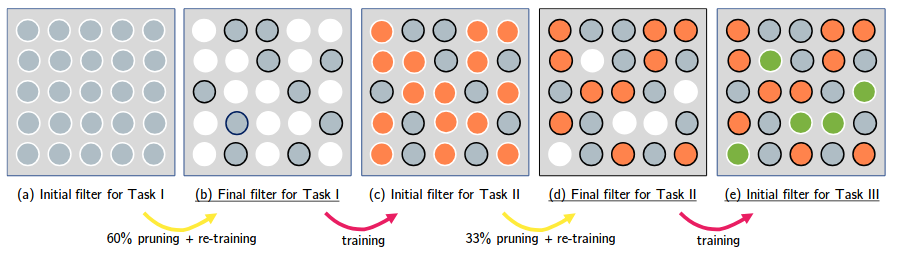
\includegraphics[width=0.9
    \textwidth]{images/CL15.png}
    \label{fig:MHA2}
\end{figure}

\subsection{Example: PackNet with Three Tasks}

Suppose we have a neural network with a large number of parameters, and we want to train it
sequentially on \textbf{three tasks}: Task~A, Task~B, and Task~C.

\vspace{0.3cm}
\hrule
\vspace{0.15cm}

\textbf{Step 1 --- Train on Task A and Prune the Network}

$\rightarrow$ We train the full network on Task~A until it achieves good performance.

$\rightarrow$ After training, we identify the most important weights for Task~A (e.g., using
magnitude-based criteria or other importance measures).

$\rightarrow$ We prune a fraction of the network’s weights that are \textbf{less important}
for Task~A (for example, pruning 60\% of the weights).

$\rightarrow$ The remaining weights, which are crucial for Task~A, are \textbf{frozen} and
cannot be updated anymore.

\vspace{0.3cm}
\hrule

\vspace{0.3cm}

\textbf{Step 2 --- Train on Task B}

$\rightarrow$ The network is retrained to recover any performance lost due to pruning.

$\rightarrow$ The \textbf{freed weights} resulting from the pruning process are used to train
the network on Task~B.

$\rightarrow$ Frozen weights from Task~A ensure that performance on Task~A is preserved.

$\rightarrow$ After training Task~B, the same procedure can be repeated: less important weights
are pruned and important ones are frozen.

\vspace{0.3cm}
\hrule
\vspace{0.3cm}

\textbf{Step 3 --- Train on Task C}

$\rightarrow$ The remaining available parameters are now used to learn Task~C.

$\rightarrow$ Weights frozen after Tasks~A and~B prevent forgetting of the previously learned
tasks.

\vspace{0.3cm}
\hrule
\vspace{0.3cm}

\textbf{Result}

$\rightarrow$ Each task is learned sequentially within the \textbf{same network}, without
catastrophic forgetting.

$\rightarrow$ Parameters are efficiently reused: only unimportant weights are reallocated for
new tasks.

$\rightarrow$ Memory overhead is minimal compared to methods that allocate a new network for
each task (e.g., Progressive Neural Networks).

\vspace{0.3cm}
\hrule
\vspace{0.3cm}

\textbf{Intuition}: Think of the network as a \emph{packing container}: Task~A fills some space, then pruning frees
unused slots. Task~B occupies the freed slots, and so on. Each task gets its own dedicated
``section'' in the same network, while the old sections remain intact.

\textbf{Inference Step in PackNet}:

(1) \textbf{Identify the task of the example}: In PackNet, \textbf{task identity is required at
test time}. The model must know which task the input belongs to (Task~A, Task~B, or Task~C).

(2) \textbf{Select the correct subset of weights}: Only the parameters assigned to the
corresponding task are activated. Weights frozen for other tasks remain unchanged.

(3) \textbf{Forward pass}: The input is processed through the network using only the relevant
parameters for the selected task.

(4) \textbf{Output}: The network produces the prediction for that task. Since weights from
previous tasks are frozen, the model does not forget how to solve earlier tasks.
